\begin{flushright} {\tiny {\color{gray} chapter3.tex}} \end{flushright}

\subsection{Some maths} \begin{flushright} {\tiny {\color{gray} maths.tex}} \end{flushright}
%~~~~~~~~~~~~~~~~~~~~~~~~~~~~~~~~~~~~~~~~~~~~~~~~~~~~~~~~~~~~~~~~~~~~~~~~~~~~~~~~~~~~~~~~~~~~~~~~~~

%----------------------------------------------------
\subsection{About vectors}

\begin{remark}
In this document I have chosen to (when possible) use the notation $\vec{a}$
to denote a vector and ${\bm a}$ to denote a tensor/matrix. More often than not 
the same notation ${\bm a}$ is used for both in the literature.
\end{remark}

In mathematics, physics and engineering, a Euclidean vector or simply a vector 
is a geometric object that has magnitude (or length) and direction. 
Many algebraic operations on real numbers such as addition, subtraction, multiplication, 
and negation have close analogues for vectors.

Let $\vec{v}$ be a vector in 3D space. 
Its Euclidean norm (or magnitude) is given in a coordinate-free way by 
\[
|\vec{v}|:=\sqrt{\vec{v}\cdot\vec{v}}
\]
This definition makes use of the dot product, see next section.
The Euclidean norm is also called the $L_2-$norm, or $2-$norm. It is also 
sometimes noted $||\cdot ||_2$. 

In Cartesian coordinates the vector $\vec{v}$ is given by
\[
\vec{v}=
\left(
\begin{array}{c}
v_x \\ v_y \\ v_z
\end{array}
\right)
=
v_x \vec{e}_x + 
v_y \vec{e}_y + 
v_z \vec{e}_z 
\qquad
\text{with}
\qquad
\vec{e}_x=
\left(
\begin{array}{c}
1 \\ 0 \\ 0
\end{array}
\right)
\quad
\vec{e}_y=
\left(
\begin{array}{c}
0 \\ 1 \\ 0
\end{array}
\right)
\quad
\vec{e}_z=
\left(
\begin{array}{c}
0 \\ 0 \\ 1
\end{array}
\right)
\]
Its norm then simply writes
\[
|\vec{v}| = \sqrt{v_x^2 + v_y^2 + v_z^2}
\]

A unit vector is any vector with a length of one. 
A vector of arbitrary length can be divided by its length to create a unit vector.
If $\vec{a}$ is a vector, the corresponding unit vector is often denoted
\[
\vec{e}_a = \frac{\vec{a}}{|\vec{a}|}
\]


%---------------------------------------------------------------
\subsection{dot products, cross products and dyadic products}

The {\bf dot product} (or sometimes called inner product, or even scalar product) of two vectors is denoted by 
$\vec{a}\cdot \vec{b}$ and is defined as:
\[
\vec{a}\cdot \vec{b} = |\vec{a}| \; |\vec{b}| \; \cos\theta
\]
where $\theta$  is the measure of the angle between $\vec{a}$ and ${b}$.

\todo[inline]{FIGURE}

In Cartesian coordinates the dot product can also be defined as the sum 
of the products of the components of each vector as
\[
\vec{a}\cdot\vec{b} = a_xb_x + a_yb_y + a_zb_z  
\]
The dot product can also be interpreted as an answer to the question ``how similar are vectors $\vec{a}$
and $\vec{b}$ in magnitude and direction?'' Indeed, if $\vec{a}=\vec{b}$ then $\theta=0$ and $\cos\theta=1$, while if 
$\vec{a}$ is perpendicular to $\vec{b}$, then $\theta=\pi/2$, $\cos\theta=0$ and $\vec{a}\cdot \vec{b}=0$. 

In Cartesian coordinates, we find that 
\[
\vec{v} \cdot \vec{e}_x 
= (v_x \vec{e}_x + v_y \vec{e}_y + v_z \vec{e}_z ) \cdot \vec{e}_x
= v_x \underbrace{\vec{e}_x \cdot \vec{e}_x}_{=1}
+ v_y \underbrace{\vec{e}_y \cdot \vec{e}_x}_{=0}
+ v_z \underbrace{\vec{e}_z \cdot \vec{e}_x}_{=0} 
=v_x
\]
In this case the interpretation of $\vec{v} \cdot \vec{e}_x$ could be ``how much of $\vec{v}$
is in the direction $\vec{e}_x$''.

The {\bf cross product} (also  called the vector product or outer product) of two vectors is also a vector.
It is denoted $\vec{a} \times \vec{b}$ and defined as 
\[
\vec{c} = \vec{a} \times \vec{b} = |\vec{a}| \; |\vec{b}|\; \sin\theta \; \vec{n}
\]
where $\theta$  is the measure of the angle between $\vec{a}$ and ${b}$ and
and $\vec{n}$ is a unit vector perpendicular to both $\vec{a}$ and $\vec{b}$ 
which completes a right-handed system.

\todo[inline]{FIGURE}

The norm of the cross product, say $|\vec{c}|=|\vec{a} \times \vec{b}|$, is actually the 
area of the parallelogram having $\vec{a}$ and $\vec{b}$ as sides.

Also note that $\vec{a} \times \vec{b} = - \vec{b} \times \vec{a}$ (think about the direction of the 
normal vector in each case). In Cartesian coordinates the cross product can be written as
\[
\vec{a} \times \vec{b} = (a_yb_z-a_zb_y) \vec{e}_x + (a_zb_x-a_xb_z) \vec{e}_y + (a_xb_y-a_yb_x) \vec{e}_z  
\]

Finally, let us look at the {\bf dyadic product} of two vectors $\vec{a}$ and $\vec{b}$ which denoted by
$\vec{a}\; \vec{b}^T$ (juxtaposed; no symbols, multiplication signs, crosses, dots, etc...). The 
result is a tensor:
\[
\vec{a}=
\left(
\begin{array}{c}
a_x \\ a_y \\ a_z
\end{array}
\right),
\qquad
\vec{b}=
\left(
\begin{array}{c}
b_x \\ b_y \\ b_z
\end{array}
\right),
\qquad\qquad
\vec{a}\vec{b}^T 
=
\left(
\begin{array}{c}
a_x \\ a_y \\ a_z
\end{array}
\right)
(b_x \; b_y \; b_z)
=
\left(
\begin{array}{ccc}
a_x b_x & a_xb_y & a_xb_z \\
a_y b_x & a_yb_y & a_yb_z \\
a_z b_x & a_zb_y & a_zb_z 
\end{array}
\right)
\]

In conclusion the dot product yields a scalar, the cross product yields a vector and the dyadic 
product yields a tensor. 






%---------------------------------------------------------------
\subsection{Rotation matrix}

After much confusion, \url{https://mathworld.wolfram.com/RotationMatrix.html}
is a source of clarity: one must be careful when speaking of 'rotation matrix'.
Indeed, there are two possible conventions: rotation of the axes, and rotation 
of the object relative to fixed axes.

We consider in $\R^2$ the matrix ${\bm R}$ that rotates a given vector $\vec{v}$
by a counterclockwise angle $\theta$ in a fixed coordinate system.
It writes
\[
{\bm R}=
\left(
\begin{array}{cc}
\cos\theta & -\sin \theta \\
\sin\theta & \cos\theta
\end{array}
\right)
\]
with $\vec{v}'={\bm R}\cdot \vec{v}$.

On the other hand, consider the matrix that rotates the coordinate system through 
a counterclockwise angle $\theta$. The coordinates of the fixed vector $\vec{v}$ in the rotated 
coordinate system are now given by a rotation matrix which is the transpose of 
the fixed-axis matrix and, as can be seen in the above diagram, is equivalent to rotating 
the vector by a counterclockwise angle of $\theta$ relative to a fixed set of axes, giving 
\[
{\bm R}=
\left(
\begin{array}{cc}
\cos\theta & \sin \theta \\
-\sin\theta & \cos\theta
\end{array}
\right)
\]
In the following example we start from $\vec{v}=(2,1)$. If we rotate the vector by 90\si{\degree}, 
the rotation matrix is given by 
\[
{\bm R}=
\left(
\begin{array}{cc}
0 & -1 \\ 1 & 0 
\end{array}
\right)
\]
so that $\vec{v}'=(-1,2)$. 
If we rotate the axis by 90\si{\degree}, the 
rotation matrix is given by 
\[
{\bm R}=
\left(
\begin{array}{cc}
0 & 1 \\ -1 & 0 
\end{array}
\right)
\]
and the coordinates of the resulting vector are $\vec{v}'=(1,-2)$.

\begin{flushright} {\tiny {\color{gray} (rotation\_matrix.tex)}} \end{flushright}
%~~~~~~~~~~~~~~~~~~~~~~~~~~~~~~~~~~~~~~~~~~~~~~~~~~~~~~~~~~~~~~~~~~~~~~~~~~~~~~~~~~~~~~~~~~~~~~~~~~

\begin{center}
\begin{tikzpicture}
%\draw[step=1cm,gray,very thin] (0,0) grid (16,7); %background grid

\draw[->,thick] (1,3)--(3,3);
\draw[->,thick] (1,3)--(1,5);
\node[] at (3,2.75) {\small $x$};
\node[] at (0.75,5) {\small $y$};
\draw[->,thick,color=blue] (1,3)--(3,4);
\node[] at (3.75,4) {\small $\vec{v}=(2,1)$};

\draw[->,thick] (5.5,4)--(7.5,5.5);
\draw[->,thick] (5.5,4)--(7.5,2.5);

\node[] at (7,4) {\small $\theta=90^o$};

\node[rotate=37] at (6.5,5.1) {\small rotate vector};
\node[rotate=-37] at (6.5,2.9) {\small rotate axis system};

\draw[->,thick] (10,4.5)--(12,4.5);
\draw[->,thick] (10,4.5)--(10,6.5);
\node[] at (12,4.25) {\small $x$};
\node[] at (9.75,6.5) {\small $y$};
\draw[->,thick,color=blue] (10,4.5)--(9,6.5);
\node[] at (8.8,6.8) {\small $\vec{v}'=(-1,2)$};

\draw[->,thick] (12,1)--(12,3);
\draw[->,thick] (12,1)--(10,1);
\node[] at (12,3.25) {\small $x$};
\node[] at (9.75,1) {\small $y$};
\draw[->,thick,color=blue] (12,1)--(14,2);
\node[] at (14,2.25) {\small $\vec{v}'=(1,-2)$};

\end{tikzpicture}
\end{center}





\subsection{Units} 
\begin{center}
\begin{tabular}{lll}
\hline
Symbol & meaning & unit \\
\hline
\hline
$t$ & Time & s \\
$x,y,z$ & Cartesian coordinates & m \\
$r,\theta$ & Polar coordinates & m,-\\
$r,\theta, z$ & Cylindrical coordinates & m,-,m\\
$r,\theta,\phi$ & Spherical coordinates & m,-,- \\
${\vec \upnu}=(u,v,w)$ & velocity vector & m$\cdot$ s$^{-1}$\\
${\vec u}$ & displacement vector & m \\
$\rho$ & mass density & kg/m$^3$ \\
$\eta$ & dynamic viscosity &  Pa$\cdot$ s \\
$\lambda$ & penalty parameter & Pa$\cdot$ s \\
$T$ & temperature & K \\
${\vec \nabla}$ & gradient operator & m$^{-1}$ \\
${\vec \nabla}\cdot$ & divergence operator & m$^{-1}$ \\
$p$ & pressure & Pa\\
$\dot{\bm \varepsilon}({\vec \upnu})$ & strain rate tensor & s$^{-1}$ \\
$\dot{\bm \varepsilon}^d({\vec \upnu})$ & deviatoric strain rate tensor & s$^{-1}$ \\
$\alpha$ & thermal expansion coefficient & K$^{-1}$ \\
$k$ & thermal conductivity & W/(m $\cdot$ K) \\
$C_p$ & Heat capacity & J/K \\
$H$ & intrinsic specific heat production & W/kg\\
$\beta_T$ & isothermal compressibility & Pa$^{-1}$  \\
${\bm \tau}$ & deviatoric stress tensor & Pa \\
${\bm \sigma}$ & full stress tensor & Pa \\
\hline
\end{tabular}
\end{center}

 %----------------------------------------------------------
\subsection{Coordinate systems} \begin{flushright} {\tiny {\color{gray} coordinate\_systems.tex}} \end{flushright}
%~~~~~~~~~~~~~~~~~~~~~~~~~~~~~~~~~~~~~~~~~~~~~~~~~~~~~~~~~~~~~~~~~~~~~~~~~~~~~~~~~~~~~~~~~~~~~~~~~~

\begin{center}
\includegraphics[width=6cm]{images/polarbear}
\end{center}

%........................................
\subsubsection{Cartesian coordinates}
\index{general}{Gradient Operator in Cartesian Coordinates}
\index{general}{Divergence Operator in Cartesian Coordinates}
\index{general}{Laplace Operator in Cartesian Coordinates}
\index{general}{Path Increment in Cartesian Coordinates}

The unit vectors along the $x$, $y$ and $z$ axis are 
$\vec{e}_x$, $\vec{e}_y$ and $\vec{e}_z$ respectively.

\begin{flushright} {\tiny {\color{gray} (tikz\_cartesian\_coordinates.tex)}} \end{flushright}
%~~~~~~~~~~~~~~~~~~~~~~~~~~~~~~~~~~~~~~~~~~~~~~~~~~~~~~~~~~~~~~~~~~~~~~~~~~~~~~~~~~~~~~~~~~~~~~~~~~
\begin{center}
\begin{tikzpicture}
%\draw[step=0.5cm,gray,very thin] (0,0) grid (4,4); %background grid

\draw [thick,->] (1.5,2) -- (3.5,2);
\draw [thick,->] (1.5,2) -- (1.5,4);
\draw [thick,->] (1.5,2) -- (0.5,0.5);

\node[] at (0.75,0.25) {$x$};
\node[] at (3.75,2) {$y$};
\node[] at (1.75,3.75) {$z$};

\draw[>=triangle 45, line width=0.3mm, ->] (1.5,2) -- (2.5,2) ;   
\node[] at (2,1.7) {$\vec{e}_x$};

\draw[>=triangle 45, line width=0.3mm, ->] (1.5,2) -- (1.5,3) ;   
\node[] at (1.9,2.75) {$\vec{e}_y$};

\draw[>=triangle 45, line width=0.3mm, ->] (1.5,2) -- (1,1.25) ;   
\node[] at (1.25,1.1) {$\vec{e}_z$};

\end{tikzpicture}
\end{center}


\noindent Any vector can then be written
\[
{\vec V}  = V_x {\vec e}_x  + V_y {\vec e}_y + V_z \vec{e}_z
\]
The gradient of a function $f$ is 
\[
\vec{\nabla} f= \text{grad }f= 
\frac{\partial f}{\partial x}\; \vec{e}_x +
\frac{\partial f}{\partial y}\; \vec{e}_y +
\frac{\partial f}{\partial z}\; \vec{e}_z,
\]
the divergence of a vector $\vec{V}$ is
\[
\vec{\nabla}\cdot \vec{V} = 
\frac{\partial V_x}{\partial x}+
\frac{\partial V_y}{\partial y}+
\frac{\partial V_z}{\partial z}
\]
and the Laplace operator of a function $f$ is:
\[
\Delta f = 
\frac{\partial^2 f}{\partial x^2} + 
\frac{\partial^2 f}{\partial y^2} + 
\frac{\partial^2 f}{\partial z^2}  
\]
Finally the path increment is
\[
d\vec{r} = dx \; {\vec e}_x  + dy\; {\vec e}_y + dz \; \vec{e}_z
\]
and the volume element is 
\[
dV=dx\; dy \; dz
\]

%........................................
\subsubsection{Polar coordinates}

We have $r>0$ and $\theta=[0,2\pi[$, defined in the $(x,y)-$plane.

\begin{flushright} {\tiny {\color{gray} (tikz\_polar\_coordinates.tex)}} \end{flushright}
%~~~~~~~~~~~~~~~~~~~~~~~~~~~~~~~~~~~~~~~~~~~~~~~~~~~~~~~~~~~~~~~~~~~~~~~~~~~~~~~~~~~~~~~~~~~~~~~~~~
\begin{center}
\begin{tikzpicture}
%\draw[step=0.5cm,gray,very thin] (0,0) grid (4.5,4); %background grid

\draw [thick,->] (1,1) -- (3.5,1);
\draw [thick,->] (1,1) -- (1,3.5);

\node[] at (3.5,0.75) {$x$};
\node[] at (0.6,3.5) {$y$};

\draw[>=triangle 45, line width=0.3mm, ->] (1,1) -- (2,1) ;   
\node[] at (1.6,0.75) {$\vec{e}_x$};

\draw[>=triangle 45, line width=0.3mm, ->] (1,1) -- (1,2) ;   
\node[] at (0.6,1.7) {$\vec{e}_y$};

\draw [-] (1,1) -- (3,2);

\draw[>=triangle 45, line width=0.3mm, ->] (3,2) -- (4,2.5) ;   
\node[] at (4.25,2.5) {$\vec{e}_r$};

\draw[>=triangle 45, line width=0.3mm, ->] (3,2) -- (2.5,3) ;   
\node[] at (2.5,3.25) {$\vec{e}_\theta$};


\node[] at (2.2,1.75) {$r$};
\node[] at (2.25,1.3) {$\theta$};

\draw[->] (2,1) arc (0:22.5:1.25);

\end{tikzpicture}
\end{center}


\noindent The relation between the unit vector in Cartesian and Polar/Cylindrical coordinates
is given by:
\[
\left(
\begin{array}{c}
{\vec e}_{r} \\
{\vec e}_{\theta} \\
\end{array}
\right)
=
\left(
\begin{array}{cc}
\cos \theta & \sin \theta \\
-\sin \theta & \cos \theta
\end{array}
\right)
\cdot
\left(
\begin{array}{c}
{\vec e}_{x} \\
{\vec e}_{y} \\
\end{array}
\right)
\]
which should be read:
\begin{eqnarray}
{\vec e}_{r}      &=& \cos\theta \; {\vec e}_{x} + \sin\theta \;  {\vec e}_{y} \nn\\
{\vec e}_{\theta} &=& -\sin\theta \; {\vec e}_{x} + \cos\theta \;  {\vec e}_{y} 
\end{eqnarray}
Note that this $2\times 2$ matrix is a 
rotation matrix\footnote{\url{https://en.wikipedia.org/wiki/Rotation_matrix}}
corresponding to an angle $-\theta$. The inverse of this matrix always exists 
(we can always counter-rotate) and it then yields
\[
\left(
\begin{array}{c}
{\vec e}_{x} \\
{\vec e}_{y} \\
\end{array}
\right)
=
\left(
\begin{array}{cc}
\cos \theta & -\sin \theta \\
\sin \theta & \cos \theta
\end{array}
\right)
\cdot
\left(
\begin{array}{c}
{\vec e}_{r} \\
{\vec e}_{\theta} \\
\end{array}
\right)
\]
so that for any vector ${\vec V}$
\begin{eqnarray}
{\vec V} 
&=& V_x {\vec e}_x  + V_y {\vec e}_y \nonumber\\
&=& V_x [(\cos \theta) {\vec e}_r - (\sin \theta) {\vec e}_\theta]  + 
    V_y [(\sin \theta) {\vec e}_r + (\cos \theta){\vec e}_\theta] \nonumber\\
&=& [V_x (\cos \theta) + V_y (\sin \theta)] {\vec e}_r +
[- V_x(\sin \theta) + V_y (\cos \theta)]{\vec e}_\theta \nn\\
&=& V_r \vec{e}_r  + V_\theta \vec{e}_\theta \nn
\end{eqnarray}
with
\begin{eqnarray}
V_r &=& V_x \cos \theta + V_y \sin \theta \nn\\
V_\theta &=& - V_x \sin \theta + V_y \cos \theta \nn
\end{eqnarray}
Finally the path increment is
\[
d\vec{r} = dr \; {\vec e}_r  + r \sin\theta d\theta \; {\vec e}_\theta
\]
and the volume element is 
\[
dV= r dr \; d\theta
\]

The gradient, divergence and Laplacian formulae are given in the following section.

\index{general}{Path Increment in Polar Coordinates}

%...........................................................
\subsubsection{Cylindrical coordinates \label{ss:cylcoord}}

%Redo with tikz
\begin{center}
\includegraphics[width=4cm]{images/cylindrical}\\
{\captionfont Cylindrical coordinates}
%https://tutorial.math.lamar.edu/classes/calcii/CylindricalCoords.aspx 
\end{center}

\[
{\vec V} 
= V_r \; \vec{e}_r  + V_\theta \; \vec{e}_\theta + V_z \; \vec{e}_z
\]
We have 
\begin{eqnarray}
x &=& r \; \cos\theta \nn\\
y &=& r \; \sin \theta \nn\\\ 
r &=& \sqrt{x^2+y^2} \nn
\end{eqnarray}

Let $f(r,\theta)$ be a function of the spatial coordinates. It s gradient is then
\[
\vec \nabla f
= \frac{\partial f}{\partial r} \; \vec{e}_r 
+ \frac{1}{r} \frac{\partial f}{\partial \theta} \; \vec{e}_\theta
+ \frac{\partial f}{\partial r} \; \vec{e}_z
\]
The divergence of a vector field $\vec{V}$ is 
\[
\vec\nabla \cdot \vec{V} 
= \frac{1}{r} \frac{\partial }{\partial r} (r V_r) 
+ \frac{1}{r} \frac{\partial V_\theta}{\partial \theta} 
+ \frac{\partial V_z}{\partial z}
\]
and the Laplacian of $f$ is
\[
\Delta f = \frac{1}{r} \frac{\partial }{\partial r} \left( r \frac{\partial f}{\partial r} \right)
+ \frac{1}{r^2} \frac{\partial^2 f}{\partial \theta^2} 
+ \frac{\partial^2 f}{\partial z^2} 
\]
Finally the path increment is
\[
d\vec{r} = dr \; {\vec e}_r  + r \sin\theta d\theta \; {\vec e}_\theta + dz \; \vec{e}_z
\]
and the volume element is 
\[
dV= r dr \; d\theta \; dz
\]
\index{general}{Gradient Operator in Cylindrical Coordinates}
\index{general}{Divergence Operator in Cylindrical Coordinates}
\index{general}{Laplace Operator in Cylindrical Coordinates}
\index{general}{Path Increment in Cylindrical Coordinates}

\begin{remark} 
Cylindrical coordinates can also be denoted by $(\rho,\theta)$, $(r,\phi)$ or even $(\rho,\phi)$.
They are sometimes called "cylindrical polar coordinates" or "polar cylindrical coordinates".
\end{remark}

%........................................
\subsubsection{Spherical coordinates \label{ss:sphercoord}}

On the following figure are represented the three Cartesian axis, 
a point and its spherical coordinates $r,\theta,\phi$:
\begin{center}
\includegraphics[width=5cm]{images/sphcoord}\\
{\captionfont Spherical coordinates as commonly used in physics:\\ polar angle $\theta$, and azimuthal angle $\phi$.} 
\end{center}
In this case $\theta\in[0:\pi]$ and $\phi\in]-\pi:\pi]$ and we have the following relationships:
\begin{eqnarray}
r &=& \sqrt{x^2+y^2+z^2} \\
\theta &=& \arccos (z/r) \\
\phi &=& \arctan (y/x) \\
x &=& r \sin \theta \cos \phi \\
y &=& r \sin\theta \sin\phi \\
z &=& r \cos\theta 
\end{eqnarray}
The inverse tangent used to compute $\phi$ must be suitably defined, 
taking into account the correct quadrant of $(x,y)$,
which is why the atan2 intrinsic function is used in \textsc{FORTRAN} for example.    
This is often written as follows:
\begin{eqnarray}
\theta &=& \arctan \left(\sqrt{x^2+y^2},z\right) \\
\phi &=& \arctan (y,x) 
\end{eqnarray}
where we formally take advantage of the two argument arctan
function to eliminate quadrant confusion.

The path increment is expressed as:

\begin{equation}
d\vec{r} = dr \; \vec{e}_r + r d\theta \; \vec{e}_\theta + r \sin\theta d\phi \; \vec{e}_\phi
\end{equation}
The gradient of a function $f(r,\theta,\phi)$ is 
\begin{equation}
\vec\nabla f= \frac{\partial f}{\partial r} \; \vec{e}_r
+ \frac{1}{r} \frac{\partial f}{\partial \theta} \; \vec{e}_\theta 
+ \frac{1}{r \; \sin\theta} \frac{\partial f}{\partial \phi} \;  \vec{e}_\phi
\end{equation}
The divergence of a vector $\vec{V}$ is
\begin{equation}
\vec\nabla\cdot \vec{V}=
\frac{1}{r^2} \frac{\partial}{\partial r} \left(r^2 V_r \right) 
+
\frac{1}{r \sin\theta} \frac{\partial}{\partial \theta} (V_\theta \sin\theta)
+
\frac{1}{r \sin\theta} \frac{\partial V_\phi}{\partial \phi}=0
\label{eq:divsc}
\end{equation}
The Laplacian of function $f$ is given by: \index{general}{Laplacian}
\begin{equation}
\Delta f= \vec\nabla \cdot\vec\nabla f= \vec\nabla^2 f
=
\frac{1}{r^2}\frac{\partial}{\partial r} \left( r^2 \frac{\partial f}{\partial r} \right)
+\frac{1}{r^2 \sin\theta} \frac{\partial}{\partial \theta} \left( \sin\theta \frac{\partial f}{\partial \theta} \right)
+\frac{1}{r^2 \sin^2\theta}  \frac{\partial^2 f}{\partial \phi^2}
\end{equation}

In geography one uses latitude and longitude, represented hereunder:
\begin{center}
\includegraphics[width=10cm]{images/map.jpg}
\end{center}
\begin{itemize}
\item Latitude  $\in[-90:90]$,   or $\in[-\pi/2:\pi/2]$ 
\item Longitude $\in]-180:180]$, or $\in]-\pi:\pi]$ 
\end{itemize}

Since the colatitude is the complementary angle of the latitude, 
i.e. the difference between 90 and the latitude, 
where southern latitudes are denoted with a minus sign,
$\theta$ as shown above is actually is the colatitude.
The colatitude is shown in red on the following figure: 
\index{general}{Colatitude}
\begin{center}
\includegraphics[width=3cm]{images/colatitude}
\end{center}

The volume of a sphere of radius $R$ is easily obtained by computing 
\begin{eqnarray}
V_{sphere} 
&=& \iiint_{sphere} dV \nn\\
&=& \int_0^R r^2 dr \int_0^\pi \sin\theta d\theta \int_0^{2\pi} d\phi  \nn\\
&=& \frac{1}{3}R^3  \cdot 2 \cdot 2\pi \nn\\
&=& \frac{4}{3}\pi R^3 
\end{eqnarray}
\index{general}{Volume of a Sphere}

The volume of a spherical shell of inner radius $R_i$ and outer radius $R_o$
is equally easily obtained by computing 

\begin{eqnarray}
V_{shell}
&=& \iiint_{shell} dV \nn\\
&=& \int_{R_i}^{R_o} r^2 dr \int_0^\pi \sin\theta d\theta \int_0^{2\pi} d\phi  \nn\\
&=& \frac{1}{3}(R_o^3-R_i^3)  \cdot 2 \cdot 2\pi \nn\\
&=& \frac{4}{3}\pi (R^3_o -R^3_i)
\end{eqnarray}
\index{general}{Volume of a Spherical shell}


\noindent The spherical unit vectors are related to the Cartesian unit vectors by:
\[
\left(
\begin{array}{c}
\vec{e}_{r} \\ \vec{e}_\theta \\ \vec{e}_\phi
\end{array}
\right)
=
\left(
\begin{array}{ccc}
\sin\theta \cos\phi & \sin\theta\sin\phi & \cos\theta  \\
\cos\theta \cos\phi & \cos\theta\sin\phi & -\sin\theta \\
-\sin\phi & \cos\phi & 0
\end{array}
\right)
\left(
\begin{array}{c}
\vec{e}_{x} \\ \vec{e}_y \\ \vec{e}_z
\end{array}
\right)
\]
and the Cartesian unit vectors are related to the spherical unit vectors by

\[
\left(
\begin{array}{c}
\vec{e}_{x} \\ \vec{e}_y \\ \vec{e}_z
\end{array}
\right)
=
\left(
\begin{array}{ccc}
\sin\theta \cos\phi & \cos\theta\cos\phi & -\sin\phi  \\
\sin\theta \sin\phi & \cos\theta\sin\phi & \cos\phi \\
\cos\theta & -\sin\theta & 0
\end{array}
\right)
\left(
\begin{array}{c}
\vec{e}_{r} \\ \vec{e}_\theta \\ \vec{e}_\phi
\end{array}
\right)
\]

\begin{eqnarray}
\vec{\upnu} 
&=& u\; \vec{e}_x + v \; \vec{e}_y + w \; \vec{e}_z \\
&=& u\; ( \sin\theta \cos\phi \; \vec{e}_r +  \cos\theta\cos\phi \;  \vec{e}_{\theta} -\sin\phi \; \vec{e}_{\phi} ) \\
&+& v\; ( \sin\theta \sin\phi \; \vec{e}_r + \cos\theta\sin\phi \; \vec{e}_\theta  +  \cos\phi \;  \vec{e}_\phi  )  \\
&+& w\; ( \cos\theta \; \vec{e}_r   -\sin\theta \; \vec{e}_\theta  ) \\
&=& v_r\; \vec{e}_r + v_\theta\; \vec{e}_\theta + v_\phi\; \vec{e}_\phi 
\end{eqnarray}
with 
\begin{eqnarray}
v_r      &=&  u \sin \theta  \cos \phi  + v \sin\theta \sin \phi + w \cos\theta \\
v_\theta &=&  u \cos\theta\cos\phi + v \cos\theta\sin\phi -w \sin\theta   \\
v_\phi   &=& -u \sin\phi  + v \cos\phi  
\end{eqnarray}

%.................................................................................................
\subsubsection{Converting tensors between Cartesian and Cylindrical bases \label{ss:convcartspher}}

\[
{\bm T}_{\tiny Cyl}=
\left(
\begin{array}{ccc}
T_{rr}       & T_{r\theta}      & T_{rz} \\
T_{\theta r} & T_{\theta\theta} & T_{\theta z} \\
T_{z r}      & T_{z \theta}     & T_{zz}
\end{array}
\right)
=
\left(
\begin{array}{ccc}
 \cos \theta&\sin \theta&0 \\
-\sin \theta&\cos \theta&0 \\
0 & 0 & 1 
\end{array}
\right)
\cdot
\left(
\begin{array}{ccc}
T_{xx} & T_{xy} & T_{xz} \\
T_{yx} & T_{yy} & T_{yz} \\
T_{zx} & T_{zy} & T_{zz} 
\end{array}
\right)
\cdot
\left(
\begin{array}{ccc}
\cos \theta & -\sin \theta&0 \\
\sin \theta &  \cos \theta&0 \\
0 & 0 & 1 
\end{array}
\right)
\]

\[
{\bm T}_{\tiny Cart}=
\left(
\begin{array}{ccc}
T_{xx} & T_{xy} & T_{xz} \\
T_{yx} & T_{yy} & T_{yz} \\
T_{zx} & T_{zy} & T_{zz} 
\end{array}
\right)
=
\left(
\begin{array}{ccc}
 \cos \theta&-\sin \theta&0 \\
\sin \theta&\cos \theta&0 \\
0 & 0 & 1 
\end{array}
\right)
\cdot
\left(
\begin{array}{ccc}
T_{rr}       & T_{r\theta}      & T_{rz} \\
T_{\theta r} & T_{\theta\theta} & T_{\theta z} \\
T_{z r}      & T_{z \theta}     & T_{zz}
\end{array}
\right)
\cdot
\left(
\begin{array}{ccc}
\cos \theta & \sin \theta&0 \\
-\sin \theta &  \cos \theta&0 \\
0 & 0 & 1 
\end{array}
\right)
\]



%.................................................................................................
\subsubsection{Converting tensors between Cartesian and Spherical bases \label{ss:convcartspher}}

Let ${\bm T}$ be a tensor
\[
{\bm T}=
\left(
\begin{array}{ccc}
T_{xx} & T_{xy} & T_{xz} \\
T_{yx} & T_{yy} & T_{yz} \\
T_{zx} & T_{zy} & T_{zz} 
\end{array}
\right)
\qquad\qquad
{\bm T}=
\left(
\begin{array}{ccc}
T_{rr}       & T_{r\theta}      & T_{r\phi} \\
T_{\theta r} & T_{\theta\theta} & T_{\theta\phi} \\
T_{\phi r}   & T_{\phi \theta}  & T_{\phi\phi}
\end{array}
\right)
\]
in the Cartesian basis (left) and the spherical basis (right).

The two sets of components are related by
\[
\left(
\begin{array}{ccc}
T_{xx} & T_{xy} & T_{xz} \\
T_{yx} & T_{yy} & T_{yz} \\
T_{zx} & T_{zy} & T_{zz} 
\end{array}
\right)
=
\left(
\begin{array}{ccc}
\sin\theta \; \cos\phi & \cos\theta \; \cos\phi & -\sin\phi \\
\sin\theta \; \sin\phi & \cos\theta \; \sin\phi &  \cos\phi \\
\cos\theta & -\sin\theta & 0 
\end{array}
\right)
\cdot
\left(
\begin{array}{ccc}
T_{rr}       & T_{r\theta}      & T_{r\phi} \\
T_{\theta r} & T_{\theta\theta} & T_{\theta\phi} \\
T_{\phi r}   & T_{\phi \theta}  & T_{\phi\phi}
\end{array}
\right)
\cdot
\left(
\begin{array}{ccc}
\sin\theta\;\cos\phi & \sin\theta\;\sin\phi & \cos\theta \\
\cos\theta\;\cos\phi & \cos\theta\;\sin\phi & -\sin\theta \\
-\sin\phi & \cos\phi & 0 
\end{array}
\right)
\]
or
\[
\left(
\begin{array}{ccc}
T_{rr}       & T_{r\theta}      & T_{r\phi} \\
T_{\theta r} & T_{\theta\theta} & T_{\theta\phi} \\
T_{\phi r}   & T_{\phi \theta}  & T_{\phi\phi}
\end{array}
\right)
=
\left(
\begin{array}{ccc}
\sin\theta \; \cos\phi & \sin\theta \; \sin\phi & \cos\theta \\
\cos\theta \; \cos\phi & \cos\theta \; \sin\phi & -\sin\theta \\
-\sin\phi & \cos\phi & 0 
\end{array}
\right)
\cdot
\left(
\begin{array}{ccc}
T_{xx} & T_{xy} & T_{xz} \\
T_{yx} & T_{yy} & T_{yz} \\
T_{zx} & T_{zy} & T_{zz} 
\end{array}
\right)
\cdot
\left(
\begin{array}{ccc}
\sin\theta\;\cos\phi & \cos\theta\;\cos\phi & -\sin\phi \\
\sin\theta\;\sin\phi & \cos\theta\;\sin\phi & \cos\phi \\
\cos\theta & -\sin\theta & 0
\end{array}
\right)
\]
If we now assume that the tensor ${\bm T}$ is symmetric (e.g. stress tensor, strain rate tensor),
then there are only 6 independent terms.

 \label{ss:coordsys} %-------------------
\subsection{A continuum mechanics primer} %--------------------------------------------------------
\begin{flushright} {\tiny {\color{gray} continuum\_mechanics.tex}} \end{flushright}
%~~~~~~~~~~~~~~~~~~~~~~~~~~~~~~~~~~~~~~~~~~~~~~~~~~~~~~~~~~~~~~~~~~~~~~~~~~~~~~~~~~~~~~~~~~~~~~~~~~

{\sl Contains contributions by W. Spakman} \index{contributors}{W. Spakman}

%......................................................................
\subsubsection{Forces}

In continuum mechanics we make a distinction between two broad classes of forces:
\begin{itemize}
\item Body forces defined as force per unit volume (N/m$^3$): gravity, electro-magnetic forces
\item Tractions: Surface forces defined as force per unit surface area (N/m$^2$):
Contact forces, elastic forces per unit area, internal flow friction, pressure, ...\\
A traction is the surface average of all atomic forces exerted by
atoms on the one side on atoms on the other side of the surface.
For real-Earth processes, internal tractions are ultimately caused by
the body forces, usually gravity.


Existing mantle flow(i.e. flow that is forced elsewhere) can exert
tractions (shear stresses) on the subducting slab or for instance at
the base of lithosphere plates.
In HPT-laboratory experiments external tractions (pressure, shear
traction) are applied to a rock sample, which cause internal
tractions to balance the exerted forces.

\begin{center}
\includegraphics[width=6cm]{images/contmech/spak1}
\end{center}
\end{itemize}

%......................................................................
\subsubsection{Stress tensor and tractions}\label{sec:stresstensor}
\index{general}{Stress Tensor} 
\index{general}{Normal Stress} 
\index{general}{Shear Stress} 
\index{general}{Stress Vector} 
\index{general}{Traction}

The Cauchy tensor\footnote{\url{https://en.wikipedia.org/wiki/Cauchy_stress_tensor}} 
consists of nine components $\sigma_{ij}$  that completely define the state of stress 
at a point inside a material. 
The tensor relates a unit-length direction vector $\vec{n}$ to the so-called 'stress vector' (most commonly called 'traction') $\vec{t}(\vec{n})$ across an imaginary surface perpendicular to $\vec{n}$:
\[
\vec{t}(\vec n)= {\vec n} \cdot {\bm \sigma}
\]

\begin{center}
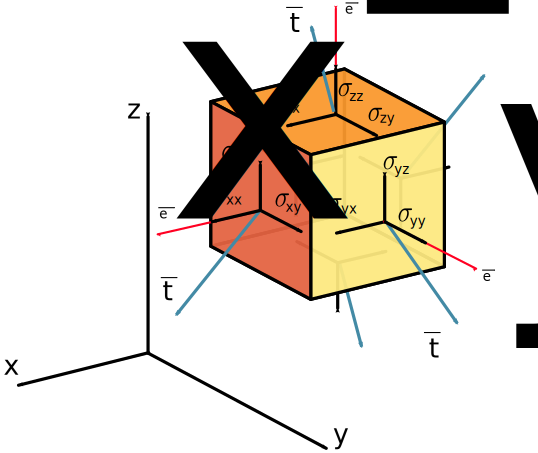
\includegraphics[width=7cm]{images/contmech/Components_stress_tensor_cartesian}\\
{\scriptsize Modified from original 
file on Wikipedia\footnote{\url{https://commons.wikimedia.org/wiki/File:Components_stress_tensor_cartesian.svg}}}
\end{center}

With respect to an orthonormal basis $\{\vec{e}_x,\vec{e}_y,\vec{e}_z\}$, the Cauchy stress tensor
is given by:
\begin{equation}
{\bm \sigma}=
\left(
\begin{array}{ccc}
\sigma_{xx} & \sigma_{xy} & \sigma_{xz} \\
\sigma_{yx} & \sigma_{yy} & \sigma_{yz} \\
\sigma_{zx} & \sigma_{zy} & \sigma_{zz} 
\end{array}
\right)
\end{equation}
The three diagonal elements are called normal stresses while the off-diagonal terms 
are called shear stresses.

One can easily prove (see for instance Section 3.3.6 of \cite{grbl09}) that the balance 
of angular momentum leads reduces to the statement that the Cauchy stress tensor 
is symmetric, i.e. ${\bm \sigma}={\bm \sigma}^T$.
Therefore, the stress state of the medium at any point and instant can be specified by only six independent parameters, rather than nine:
\begin{equation}
{\bm \sigma}=
\left(
\begin{array}{ccc}
\sigma_{xx} & \sigma_{xy} & \sigma_{xz} \\
\sigma_{xy} & \sigma_{yy} & \sigma_{yz} \\
\sigma_{xz} & \sigma_{yz} & \sigma_{zz} 
\end{array}
\right)
\qquad\qquad
\text{or sometimes}
\qquad\qquad
{\bm \sigma}=
\left(
\begin{array}{ccc}
\sigma_{x}  & \tau_{xy}  & \tau_{xz} \\
\tau_{xy}   & \sigma_{y} & \tau_{yz} \\
\tau_{xz}   & \tau_{yz}  & \sigma_{z} 
\end{array}
\right)
\end{equation}
where the elements $\sigma _{x}$, $\sigma _{y}$, $\sigma _{z}$ are called the orthogonal 
normal stresses (relative to the chosen coordinate system), and $\tau _{xy}$, $\tau _{xz}$,
$\tau _{yz}$ the orthogonal shear stresses.
As seen above, the SI units of both stress tensor and traction are \si{\newton\per\square\metre}.

In Cylindrical coordinates the stress tensor components are given by:
\begin{eqnarray}
\sigma_{rr} &=& -p + 2 \eta \frac{\partial \upnu_r}{\partial r}      \\
\sigma_{\theta\theta} &=& 
 -p + 2\eta \left( \frac{1}{r} \frac{\partial \upnu_\theta}{\partial\theta} +\frac{\upnu_r}{r} \right)    \\
\sigma_{zz} &=& -p + 2 \eta \frac{\partial \upnu_z}{\partial z}      \\
\sigma_{r\theta} &=& \eta \left( \frac{1}{r} \frac{\partial \upnu_r}{\partial \theta} 
+ \frac{\partial \upnu_\theta}{\partial r} - \frac{\upnu_\theta}{r} \right)  \\
\sigma_{rz} &=& \eta \left( \frac{\partial \upnu_r}{\partial z}  + \frac{\partial \upnu_z}{\partial r}\right) \\
\sigma_{\theta z} &=&  \eta \left(  \frac{1}{r} \frac{\partial \upnu_z}{\partial \theta}
+\frac{\partial \upnu_\theta}{\partial z}     \right) 
\end{eqnarray}
\index{general}{Stress Tensor (Cylindrical Coordinates)}

In Spherical coordinates the stress tensor components are given by:
\begin{eqnarray}
\sigma_{rr} &=& -p + 2 \eta \frac{\partial \upnu_r}{\partial r}      \\
\sigma_{\theta\theta} &=& 
 -p + 2\eta \left( \frac{1}{r} \frac{\partial \upnu_\theta}{\partial\theta} +\frac{\upnu_r}{r} \right)    \\
\sigma_{\phi\phi} &=& 
-p + 2\eta \left( \frac{1}{r \sin \theta} \frac{\partial \upnu_\phi}{\partial \phi} 
+\frac{\upnu_r}{r}  + \frac{\upnu_\theta \cot \theta}{r} \right) \\
\sigma_{r\theta} &=& \eta\left(  r \frac{\partial}{\partial r} \frac{\upnu_\theta}{r}  
+\frac{1}{r} \frac{\partial \upnu_r}{\partial\theta}   \right)\\
\sigma_{r\phi} &=& \eta \left( \frac{1}{r \sin\theta}\frac{\partial \upnu_r}{\partial \phi} 
+ r \frac{\partial}{\partial r} \frac{\upnu_\phi}{r}  \right)\\
\sigma_{\theta \phi} &=& \eta \left(
\frac{1}{r \sin\theta} \frac{\partial \upnu_\theta}{\partial\phi}
+\frac{\sin\theta}{r} \frac{\partial}{\partial \theta} \frac{\upnu_\phi}{\sin\theta}
\right) 
\end{eqnarray}
\index{general}{Stress Tensor (Spherical Coordinates)}

 %----------------------------------------------------------------------

\begin{center}
\begin{tabular}{lll}
\hline
Symbol & meaning & unit \\
\hline
\hline
$t$ & Time & s \\
$x,y,z$ & Cartesian coordinates & m \\
${\bm v}$ & velocity vector & m$\cdot$ s$^{-1}$\\
$\rho$ & mass density & kg/m$^3$ \\
$\eta$ & dynamic viscosity &  Pa$\cdot$ s \\
$\lambda$ & penalty parameter & Pa$\cdot$ s \\
$T$ & temperature & K \\
${\bm \nabla}$ & gradient operator & m$^{-1}$ \\
${\bm \nabla}\cdot$ & divergence operator & m$^{-1}$ \\
$p$ & pressure & Pa\\
$\dot{\bm \varepsilon}({\bm v})$ & strain rate tensor & s$^{-1}$ \\
$\alpha$ & thermal expansion coefficient & K$^{-1}$ \\
$k$ & thermal conductivity & W/(m $\cdot$ K) \\
$C_p$ & Heat capacity & J/K \\
$H$ & intrinsic specific heat production & W/kg\\
$\beta_T$ & isothermal compressibility & Pa$^{-1}$  \\
${\bm \tau}$ & deviatoric stress tensor & Pa \\
${\bm \sigma}$ & full stress tensor & Pa \\
\hline
\end{tabular}
\end{center}

%------------------------------------------------------------------------
\subsection{The heat transport equation - energy conservation equation}

Let us start from the heat transport equation as shown in Schubert, Turcotte and Olson \cite{scto01}:
\[
\rho C_p \frac{DT}{Dt} - \alpha T \frac{Dp}{Dt} = {\bm \nabla} \cdot k {\bm \nabla} T + \Phi + \rho H  
\]
with $D/Dt$ being the total derivatives so that 
\[
\frac{DT}{Dt} = \frac{\partial T}{\partial t} + {\bm v}\cdot {\bm \nabla}T
\quad\quad
\frac{Dp}{Dt} = \frac{\partial p}{\partial t} + {\bm v}\cdot {\bm \nabla}p
\]
Solving for temperature, this equation is often rewritten as follows:
\begin{mdframed}[backgroundcolor=blue!5]
\[
\rho C_p \frac{DT}{Dt} - {\bm \nabla} \cdot k {\bm \nabla} T =  \alpha T \frac{Dp}{Dt} + \Phi + \rho H  
\]
\end{mdframed}

A note on the shear heating term $\Phi$: In many publications, $\Phi$ 
is given by $\Phi=\tau_{ij}\partial_j u_i={\bm \tau}:{\bm \nabla}{\bm v}$.

\begin{eqnarray}
\Phi 
&=& \tau_{ij}\partial_j u_i \nonumber\\
&=& 2 \eta \dot{\varepsilon}_{ij}^d\partial_j u_i \nonumber\\
&=& 2 \eta \frac{1}{2}\left( \dot{\varepsilon}_{ij}^d\partial_j u_i + \dot{\varepsilon}_{ji}^d\partial_i u_j \right) \nonumber\\
&=& 2 \eta \frac{1}{2}\left( \dot{\varepsilon}_{ij}^d\partial_j u_i + \dot{\varepsilon}_{ij}^d\partial_i u_j \right) \nonumber\\
&=& 2 \eta  \dot{\varepsilon}_{ij}^d  \frac{1}{2}\left(\partial_j u_i + \partial_i u_j \right) \nonumber\\
&=& 2 \eta  \dot{\varepsilon}_{ij}^d   \dot{\varepsilon}_{ij} \nonumber\\
&=& 2 \eta  \dot{\bm \varepsilon}^d :  \dot{\bm \varepsilon} \nonumber\\
&=& 2 \eta  \dot{\bm \varepsilon}^d : \left( \dot{\bm \varepsilon}^d +\frac{1}{3} ({\bm \nabla}\cdot{\bm v}) {\bm 1} \right)\nonumber\\
&=& 2 \eta  \dot{\bm \varepsilon}^d : \dot{\bm \varepsilon}^d 
+ 2 \eta  \dot{\bm \varepsilon}^d : {\bm 1} ({\bm \nabla}\cdot{\bm v}) \nonumber\\ 
&=& 2 \eta  \dot{\bm \varepsilon}^d : \dot{\bm \varepsilon}^d 
\end{eqnarray}
Finally
\[
\Phi = {\bm \tau}:{\bm \nabla}{\bm v} = 2 \eta  \dot{\bm \varepsilon}^d : \dot{\bm \varepsilon}^d
= 2 \eta \left( (\dot{\varepsilon}_{xx}^d)^2 + (\dot{\varepsilon}_{yy}^d)^2 + 2(\dot{\varepsilon}_{xy}^d)^2 \right)
\]

%------------------------------------------------------------------------
\subsection{The momentum conservation equations} 

Because the Prandlt number is virtually zero in Earth science applications the Navier Stokes 
equations reduce to the Stokes equation:
\[
{\bm \nabla}\cdot {\bm \sigma} + \rho {\bm g} = 0
\]
Since 
\[
{\bm \sigma} = -p {\bm 1} + {\bm \tau}
\]
it also writes
\[
-{\bm \nabla}p + {\bm \nabla}\cdot {\bm \tau} + \rho {\bm g} = 0
\]
Using the relationship ${\bm \tau} = 2 \eta \dot{\bm \varepsilon}^d$ we arrive at 
\begin{mdframed}[backgroundcolor=blue!5]
\[
-{\bm \nabla}p + {\bm \nabla}\cdot (2 \eta \dot{\bm \varepsilon}^d ) + \rho {\bm g} = 0
\]
\end{mdframed}

%------------------------------------------------------------------------
\subsection{The mass conservation equations} 

The mass conservation equation is given by
\[
\frac{D\rho}{Dt} + \rho {\bm \nabla}\cdot{\bm v} = 0
\]
or, 
\begin{mdframed}[backgroundcolor=blue!5]
\[
\frac{\partial \rho}{\partial t} + {\bm \nabla}\cdot(\rho {\bm v}) = 0
\]
\end{mdframed}
In the case of an incompressible flow, then $\partial \rho/\partial t=0$ and 
${\bm \nabla}\rho=0$, i.e. $D\rho/Dt=0$ and the remaining equation is simply:
\[
{\bm \nabla}\cdot{\bm v} = 0
\]

\subsection{The equations in ASPECT manual}
The following is lifted off the ASPECT manual.
We focus on the system of equations in a $d=2$- or $d=3$-dimensional
domain $\Omega$ that describes the motion of a highly viscous fluid driven
by differences in the gravitational force due to a density that depends on
the temperature. In the following, we largely follow the exposition of this
material in Schubert, Turcotte and Olson \cite{scto01}.

Specifically, we consider the following set of equations for velocity $\mathbf
u$, pressure $p$ and temperature $T$:
\begin{align}
  \label{eq:stokes-1}
  -\nabla \cdot \left[2\eta \left(\dot\varepsilon(\bm v)
                                  - \frac{1}{3}(\nabla \cdot \bm v)\mathbf 1\right)
                \right] + \nabla p &=
  \rho \bm g
  &
  & \textrm{in $\Omega$},
  \\
  \label{eq:stokes-2}
  \nabla \cdot (\rho \bm v) &= 0
  &
  & \textrm{in $\Omega$},
  \\
  \label{eq:temperature}
  \rho C_p \left(\frac{\partial T}{\partial t} + \bm v\cdot\nabla T\right)
  - \nabla\cdot k\nabla T
  &=
  \rho H
  \notag
  \\
  &\quad
  +
  2\eta
  \left(\dot\varepsilon(\bm v) - \frac{1}{3}(\nabla \cdot \bm v)\mathbf 1\right)
  :
  \left(\dot\varepsilon(\bm v) - \frac{1}{3}(\nabla \cdot \bm v)\mathbf 1\right)
  \\
  &\quad
  +\alpha T \left( \bm v \cdot \nabla p \right)
  \notag
  \\
  &\quad
  &
  & \textrm{in $\Omega$},
  \notag
\end{align}
where $\dot{\bm \varepsilon}(\mathbf u) = \frac{1}{2}(\nabla \mathbf u + \nabla\mathbf
u^T)$ is the symmetric gradient of the velocity (often called the
\textit{strain rate}).%

In this set of equations, \eqref{eq:stokes-1} and \eqref{eq:stokes-2}
represent the compressible Stokes equations in which $\mathbf v=\mathbf
v(\mathbf x,t)$ is the velocity field and $p=p(\mathbf x,t)$ the pressure
field. Both fields depend on space $\mathbf x$ and time $t$. Fluid flow is
driven by the gravity force that acts on the fluid and that is proportional to
both the density of the fluid and the strength of the gravitational pull.

Coupled to this Stokes system is equation \eqref{eq:temperature} for the
temperature field $T=T(\mathbf x,t)$ that contains heat conduction terms as
well as advection with the flow velocity $\mathbf v$. The right hand side
terms of this equation correspond to
\begin{itemize}
\item internal heat production for example due to radioactive decay;
\item friction (shear) heating;
\item adiabatic compression of material;
\end{itemize}

In order to arrive at the set of equations that ASPECT solves, 
we need to 
\begin{itemize}
\item neglect the $\partial p/\partial t$. {\color{red}WHY?}
\item neglect the $\partial \rho / \partial t$ . {\color{red}WHY?}
\end{itemize}
from equations above. 

----------------------------------------

Also, their definition of the shear heating term $\Phi$ is:
\[
\Phi = k_B ({\bm \nabla}\cdot{\bm v})^2 + 2\eta \dot{\bm \varepsilon}^d:\dot{\bm \varepsilon}^d
\]
For many fluids the bulk viscosity $k_B$ is very small and is often taken to be zero, an assumption known
as the Stokes assumption: $k_B=\lambda+2\eta/3=0$. \index{bulk viscosity}
Note that $\eta$ is the dynamic viscosity and $\lambda$ the second viscosity. \index{dynamic viscosity}
\index{second viscosity}
Also, 
\[
{\bm \tau}=2\eta \dot{\bm \varepsilon} + \lambda ({\bm \nabla}\cdot{\bm v}) {\bm 1}
\]
but since $k_B=\lambda+2\eta/3=0$, then $\lambda=-2\eta/3$ so 
\[
{\bm \tau}=2\eta \dot{\bm \varepsilon} -\frac{2}{3}\eta ({\bm \nabla}\cdot{\bm v}) {\bm 1} = 2\eta \dot{\bm \varepsilon}^d
\]







\newpage
%---------------------------------
\subsection{the Boussinesq approximation: an Incompressible flow}

\index{Boussinesq}

[from aspect manual]
The Boussinesq approximation assumes that the density can be
considered constant in all occurrences in the equations with the exception of
the buoyancy term on the right hand side of \eqref{eq:stokes-1}. The primary
result of this assumption is that the continuity equation \eqref{eq:stokes-2}
will now read
\[
{\bm \nabla}\cdot{\bm v} = 0
\]
This implies that the strain rate tensor is deviatoric.
Under the Boussinesq approximation, the equations are much simplified:

\begin{align}
  \label{eq:stokes-1}
  -\nabla \cdot \left[2\eta \dot{\bm \varepsilon}(\bm v)
                \right] + \nabla p &=
  \rho \bm g
  &
  & \textrm{in $\Omega$},
  \\
  \label{eq:stokes-2}
  \nabla \cdot (\rho \bm v) &= 0
  &
  & \textrm{in $\Omega$},
  \\
  \label{eq:temperature}
  \rho_0 C_p \left(\frac{\partial T}{\partial t} + \bm v\cdot\nabla T\right)
  - \nabla\cdot k\nabla T
  &=
  \rho H
  &
  & \textrm{in $\Omega$}
\end{align}
Note that all terms on the rhs of the temperature equations have disappeared, with the exception 
of the source term.


\newpage
\subsection{Stokes equation for elastic medium}

What follows is mostly borrowed from Becker \& Kaus lecture notes.

%\begin{tabular}{|l|l|l|}
%\hline
%${\bm u}       $ & displacement vector &   \\
%${\bm \sigma}  $ & full stress tensor  & Pa\\
%${\bm \epsilon}$ & strain tensor       &   \\
%${\bm 1}       $ & unit tensor         &   \\
%${\bm f}       $ & body forces         &   \\
%\hline
%\end{tabular}

The strong form of the PDE that governs force balance in a medium is given by
\[
{\bm \nabla}\cdot{\bm \sigma}  + {\bm f} = {\bm 0}
\]
where ${\bm \sigma}$ is the stress tensor and ${\bm f}$ is a body force.

The stress tensor is related to the strain tensor through the generalised 
Hooke's law:
\begin{equation}
\sigma_{ij}=\sum_{kl}C_{ijkl}\epsilon{kl} \label{eq:one}
\end{equation}
where ${\bm C}$ is the fourth-order elastic tensor.
In the case of an isotropic material, this relationship simplifies to
\begin{equation}
\sigma_{ij}=\lambda \epsilon_{kk} \delta_{ij} + 2\mu \epsilon_{ij}
\quad\quad
or, 
\quad\quad
{\bm \sigma} = \lambda ({\bm \nabla}\cdot{\bm u})  {\bm 1} + 2\mu {\bm \epsilon}   \label{eq:two}
\end{equation}
where $\lambda$ is the Lam\'e parameter and $\mu$ is the shear modulus\footnote{It is also sometimes written $G$}.
The term ${\bm \nabla}\cdot{\bm u}$ is the isotropic dilation.

\index{Lam\'e parameter} \index{shear modulus}

The strain tensor is related to the displacement as follows: \index{strain tensor}
\[
{\bm \epsilon} = \frac{1}{2}({\bm \nabla}{\bm u} + {\bm \nabla}{\bm u}^T)
\]

The incompressibility (bulk modulus), $K$, is defined as $p=-K {\bm \nabla}\cdot{\bm u}$ 
where $p$ is the pressure with \index{bulk modulus}
\begin{eqnarray}
p&=&-\frac{1}{3}Tr({\bm \sigma}) \nonumber\\
 &=& -\frac{1}{3} [ \lambda ({\bm \nabla}\cdot{\bm u}) Tr[{\bm 1}] + 2 \mu Tr[{\bm \epsilon}]] \nonumber\\
 &=& -\frac{1}{3} [ \lambda ({\bm \nabla}\cdot{\bm u})  3  + 2 \mu  ({\bm \nabla}\cdot{\bm u}) ] \nonumber\\
 &=& -[ \lambda  + \frac{2}{3} \mu ]   ({\bm \nabla}\cdot{\bm u})  
\end{eqnarray}
so that $K=\lambda+\frac{2}{3}\mu$.

%or
%\[
%\mu=\frac{3K(1-2\nu)}{2(1+\nu)}
%\]


\paragraph{Remark}: Eq. (\ref{eq:one}) and (\ref{eq:two}) are analogous to the ones that one has to solve
in the context of viscous flow using the penalty method. In this case $\lambda$ is the penalty coefficient, 
${\bm u}$ is the velocity, and $\mu$ is then the dynamic viscosity.

%\begin{center}
%\includegraphics[width=15cm]{images/coeffs}\\
%{\small Homogeneous isotropic linear elastic materials have their elastic properties uniquely determined by any two moduli among these; thus, given any two, any other of the elastic moduli can be calculated according to these formulas.}
%\end{center}

The Lam\'e parameter and the shear modulus are also linked to $\nu$ the poisson ratio, 
and $E$, Young's modulus: \index{Poisson ratio} \index{Young's modulus}
\[
\lambda=\mu\frac{2\nu}{1-2\nu}
=\frac{\nu E}{(1+\nu)(1-2\nu)}
\quad\quad
{\rm with}
\quad\quad
E=2\mu(1+\nu)
\]
The shear modulus, expressed often in GPa, describes the material's response to shear stress.
The poisson ratio describes the response in the direction orthogonal to uniaxial stress.
The Young modulus, expressed in GPa, describes the material's strain response to uniaxial stress in the 
direction of this stress.









 %----------------------------------------------------------------------------------
\newpage
\subsection{Rheology in geodynamics} 
For now what follows only deals with viscous behavior.


\subsubsection{Linear viscous aka Newtonian} \index{Newtonian fluid}

Simply put, a Newtonian fluid is a fluid in which the viscous stresses at every point are linearly proportional 
to the local strain rate.
Mathematically speaking, this means that the fourth-order tensor ${\bm C}$ relating the viscous stress 
tensor to the strain rate tensor does not depend on the stress state and velocity of the flow.
\[
{\bm s}={\bm C} \cdot \dot{\bm \varepsilon}
\]

One very often make sthe assumption that the fluid is isotropic, i.e. its mechanical properties are the 
same along any direction. As a consequence the fourth order viscosity tensor 
${\bm C}$ is symmetric and will have only two independent real parameters: 
a bulk viscosity coefficient, that defines the resistance of the medium to gradual uniform compression; 
and a dynamic viscosity coefficient $\eta$ that expresses its resistance to gradual shearing, 
(we here neglect the so-called rotational viscosity coefficient which results from a coupling between the fluid flow and the rotation of the individual particles). %wiki



Rather logically we denote by non-Newtonian fluids with are not Newtonian, i.e. their viscosity (tensor)
depends on stress. Such fluids are part of our daily life, e.g. honey, toothpaste, paint, blood, and shampoo. 
 


%------------------------------
\subsubsection{Power-law model}
\index{Power-law model}

One of the simplest non-Newtonian viscosity model is the power-law model:
\begin{equation}
\eta = K \dot{\varepsilon}_{II}^{(n-1)/2}
\end{equation}
where $\dot{\varepsilon}_{II}$ is the second invariant of the strain rate tensor as defined in 
Section~\ref{sec:invariants}, and $n$ and $K$ are parameters. $n$ is called the power-law index.

Note that a Newtonian viscosity is recovered when $n=1$. Also $n$ and $K$ may depend on temperature
\cite[p339]{reddybook2}.


%------------------------------
\subsubsection{Carreau model}



%------------------------------
\subsubsection{Bingham model}


%------------------------------
\subsubsection{Herschel-Bulkley visco-plastic model}

The Herschel-Bulkley model is effectively a combination of the power-law model and 
a simple plastic model:
\begin{eqnarray}
{\bm s} &=& 2 \left(  K \dot{\varepsilon}^{n-1} + \frac{\tau_0}{\dot{\varepsilon}}\right)\dot{\bm \varepsilon} \qquad \text{ if } {s}_{II}>\tau_0 \\
\dot{\bm \varepsilon} &=& {\bm 0} \qquad {s}_{II} \leq \tau_0 \\
\end{eqnarray}
in which $\dot{\varepsilon}=\sqrt{\dot{\varepsilon}_{II}}$, 
$\tau_0$ is the yield stress, $K$ the consistency, and $n$ is the flow index \cite{bemj04}.
The flow index measures the degree to which the fluid is shear-thinning ($n<1$) or shear-thickening ($n>1$).
If $n=1$ and $\tau_0=0$ the model reduces to the Newtonian model. 

The term between parenthesis above is the nonlinear effective viscosity. Concretely, the implementation goes as 
follows\footnote{\url{https://en.wikipedia.org/wiki/Herschel-Bulkley_fluid}}:
\[
\eta_{eff} = 
\left\{
\begin{array}{cc}
\eta_0 & \dot{\varepsilon}\leq \dot{\varepsilon}_0 \\ 
K \dot{\varepsilon}^{n-1} + \frac{\tau_0}{\dot{\varepsilon}} & \dot{\varepsilon} \geq \dot{\varepsilon}_0
\end{array}
\right.
\]
The limiting viscosity $\eta_0$ is chosen such that 
$\eta_0 =  K \dot{\varepsilon}_0^{n-1} + \frac{\tau_0}{\dot{\varepsilon}_0}$

A large limiting viscosity means that the fluid will only flow in response to a large applied force. 
This feature captures the Bingham-type behaviour of the fluid. 
Note that when strain rates are large, the power-law behavior dominates. 

As we have seen for Bingham fluids, the equations above are not easily amenable to implementation so that 
one usually resorts to regularisation, which is a modification of the 
equations by introducing a new material parameter which controls the exponential 
growth of stress. This way the equation is valid for both yielded and unyielded areas
\cite{blmi97,papa87}:
\[
\eta_{eff} = K \dot{\varepsilon}^{n-1} + \frac{\tau_0}{\dot{\varepsilon}} [1 - \exp(-m \dot{\varepsilon})] 
\]
When the strain rate becomes (very) small a Taylor expansion of the regularisation 
term yields $1- \exp(-m \dot{\varepsilon}) \sim m \dot{\varepsilon} $ so that 
$\eta_{eff} \rightarrow m \tau_0$.

\todo[inline]{Channel flow of wikipedia with analytical solution!}


%------------------------------
\subsubsection{Dislocation creep}

%------------------------------
\subsubsection{Diffusion creep}

%------------------------------
\subsubsection{Peierls creep}



 %--------------------------------------------


\newpage
%------------------------------
\subsection{The Perzyna model}\label{sec:perzyna}
\index{general}{Perzyna Model}
\begin{flushright} {\tiny {\color{gray} perzyna.tex}} \end{flushright}
%~~~~~~~~~~~~~~~~~~~~~~~~~~~~~~~~~~~~~~~~~~~~~~~~~~~~~~~~~~~~~~~~~~~~~~~~~~~~~~~~~~~~~~~~~~~~~~~~~~


The Perzyna formulation is mentioned in \url{
https://en.wikipedia.org/wiki/Viscoplasticity}.
It is a rate-dependent plasticity formulation that was proposed in 1966 by Piotr Perzyna \cite{perz66}.
See also \url{https://neml.readthedocs.io/en/dev/vp_flow/perzyna.html}.



In what follows I make use of the approach and notations of Zienkiewicz (1974) \cite{zico74} (and all 
the 1974-75 papers that follow) and the book by Owen \& Hinton \cite{owhi}.

The total strain (rate) is divided into two parts\footnote{Zienkiewicz \cite{zico74} 
adds a third term ${\bm \varepsilon}^0$ which stands for initial/autogenous strain such as due 
to temperature changes but I neglect it in what follows.}:
\[
\dot{\bm \varepsilon} = \dot{\bm \varepsilon}^e + \dot{\bm \varepsilon}^{vp}  
\]
where ${\bm \varepsilon}^e$ stands for the elastic strain tensor and 
${\bm \varepsilon}^{vp}$ stands for the visco-plastic strain tensor.

%Since the tensors are symmetric only 6 of the 9 components are independent and 
%the above relationship is often re-written
%\[
%\vec{\varepsilon} = \vec{\varepsilon}^e + \vec{\varepsilon}^{vp}  
%\]
%with
%\[
%\vec{\varepsilon}=
%\left(
%\begin{array}{c}
%\varepsilon_{xx} \\
%\varepsilon_{yy} \\
%\varepsilon_{zz} \\
%\varepsilon_{xy} \\
%\varepsilon_{xz} \\
%\varepsilon_{yz} 
%\end{array}
%\right)
%\]
%For a linear elastic material 
%\[
%{\vec \varepsilon}^e = {\bm D}^{-1} \cdot {\vec \sigma}
%\]
%where ${\bm D}^{-1}$ is a symmetric elasticity matrix (compliance matrix).




The yield condition is given as 
\[
{\FFF}({\bm \sigma},\kappa) 
= \Psi(\bm\sigma,\dot{\bm \varepsilon}) -Y(\kappa) = 0
\]
with ${\FFF}<0$ denoting the purely elastic region, $\kappa$ is a 
history-dependent hardening/softening parameter and $Y(\kappa)$ is a static yield stress.
$\Psi$ is a function of the stress and/or strain rate invariants.

We borrow from classical viscoplasticity theory (Perzyna (1966) \cite{perz66}, Perzyna (1988) \cite{perz88}) 
the idea of a plastic potential defined as $\QQQ({\bm \sigma})$ and write
\begin{equation}
{\dot{\bm \varepsilon}}^{vp} 
= \gamma \Big\langle
\phi\left( {\FFF} \right) 
\Big\rangle
\frac{\partial \QQQ}{\partial \bm\sigma}
\end{equation}
where $\gamma$ is a positive, possibly time-dependent fluidity parameter. 
Note that sometimes the pseudo-viscosity $\bar{\eta}=\gamma^{-1}$ is defined \cite{zigo74}
so that the equation above writes:
\begin{equation}
{\dot{\bm \varepsilon}}^{vp} 
= \frac{1}{\bar{\eta}} \Big\langle
\phi\left( {\FFF} \right) 
\Big\rangle
\frac{\partial \QQQ}{\partial \bm\sigma}
\end{equation}
${\FFF}$ represents the plastic yield condition.
$\phi(x)$ is a positive scalar-valued monotonic increasing function in the range 
$x>0$ such that $\phi^{-1}(x)$ exists and possess similar properties in the same range. 
The notation $\langle \rangle$ denotes the Macaulay 
brackets\footnote{\url{https://en.wikipedia.org/wiki/Macaulay_brackets}} and stands 
for\footnote{there is a difference between 
\cite{zico74}(1974) and \cite{zico74b}(1974) wrt $>$ and $\ge$, and also 
a difference with wikipedia!} 
\begin{eqnarray}
\langle \phi(x) \rangle = \phi(x) & {\rm if} & x>0 \nonumber\\
\langle \phi(x) \rangle = 0 & {\rm if} & x\le 0 \nonumber
\end{eqnarray}
If ${\QQQ}={\FFF}$ then we speak of an {\it associative} law and if ${\QQQ} \neq {\FFF}$ 
we have a {\it non-associative} situation. 
The tensor $\frac{\partial \QQQ}{\partial \bm\sigma}$ represents the direction
of plastic flow and when ${\FFF}={\QQQ}$ it is a vector directed normal to the yield surface
at the stress point under consideration. This is potentially problematic in the 
case of the Tresca and Mohr-Coulomb yield surfaces since the normal is not well defined
along the apices of the surfaces (see Section~7.6 of \cite{owhi}).
In the non-associative case, the direction of plastic flow in the 
principal  stress space during plastic flow is not the same
as the direction of the vector normal to the yield surface.

In what follows we concentrate our attention on isotropic materials for which 
both ${\FFF}$ and ${\QQQ}$ can be defined in terms of stress invariants.

According to Zienkiewicz et al (1975) \cite{zihl75}:
\begin{displayquote}
{\color{darkgray}
One of the main stumbling blocks of the 
classical plasticity theory lay in the universal
assumption, based on Drucker's postulates (Drucker and Prager, 1952), that the plastic 
behaviour is `associated'. With the use of Mohr-Coulomb type yield envelopes to define the
limit between states of elasticity and of continuing irreversible deformation,
the associated behaviour manifestly contradicted observation and gave excessive dilation.
It became necessary therefore to extend plasticity ideas to a `non-associated'
form in which the plastic potential and yield surfaces are defined separately.}
\end{displayquote}
At the same time, it is worth remembering that these early studies mostly dealt
with plasticity in metals, and later soils, but not kilometer-scale crustal layers.

Also, the Perzyna model is not the only one, see for instance
the Duvaut-Lions viscoplastic model or the Consistency model \cite{wasd97,hesd02}.

We therefore need to look into the derivative of the plastic potential ${\QQQ}$
with respect to the stress tensor. Since the potential 
is expressed as a function of the stress invariants ${\III}_1(\bm\sigma)$,
${\III}_2(\bm\tau)$ and $\theta_L(\bm\tau)$, we then have\footnote{
The derivative of the Lod\'e angle was obtained in Section~\ref{ss:lode}}:

\begin{eqnarray}
\frac{\partial \QQQ}{\partial \bm\sigma}
&=&
\frac{\partial }{\partial \bm\sigma} \QQQ\left({\III}_1(\bm\sigma),{\III}_2(\bm\tau),\theta_{\rm L}(\bm\tau)\right)\nn\\
&=&
\frac{\partial \QQQ}{\partial {\III}_1(\bm\sigma)} 
\frac{\partial {\III}_1(\bm\sigma)}{\partial \bm\sigma} 
+
\frac{\partial \QQQ}{\partial \sqrt{{\III}_2(\bm\tau)}} 
\frac{\partial \sqrt{ {\III}_2(\bm\tau)}   }{\partial {\III}_2(\bm\tau)} 
\frac{\partial {\III}_2(\bm\tau)}{\partial \bm\sigma} 
+
\frac{\partial \QQQ}{\partial \theta_{\rm L}(\bm\tau)} 
\frac{\partial \theta_{\rm L}(\bm\tau)}{\partial \bm\sigma} \nn\\
&=&
\frac{\partial \QQQ}{\partial {\III}_1(\bm\sigma)} 
\frac{\partial {\III}_1(\bm\sigma)}{\partial \bm\sigma} 
+
\frac{\partial \QQQ}{\partial \sqrt{{\III}_2(\bm\tau)}} 
\frac{1}{2 \sqrt{ {\III}_2(\bm\tau)}   }
\frac{\partial {\III}_2(\bm\tau)}{\partial \bm\sigma} 
\nn\\
&&
-
\frac{\partial \QQQ}{\partial \theta_{\rm L}(\bm\tau)} 
\frac{\sqrt{3}}{2\cos 3\theta_{\rm L}}
\left[
-\frac32  \frac{ {\III}_3(\bm\tau)   }{ {\III}_2(\bm\tau)^{5/2}}
\; \frac{\partial {\III}_2(\bm\tau)}{\partial \bm\sigma} 
+  \frac{1}{{\III}_2(\bm\tau)^{3/2}} 
\; \frac{\partial {\III}_3(\bm\tau)}{\partial \bm\sigma} 
\right] \nn\\
&=&
\frac{\partial \QQQ}{\partial {\III}_1(\bm\sigma)} 
\; \frac{\partial {\III}_1(\bm\sigma)}{\partial \bm\sigma} 
+  
\left(\frac{\partial \QQQ}{\partial \sqrt{{\III}_2(\bm\tau)}} 
\frac{1}{2 \sqrt{ {\III}_2(\bm\tau)}   }   
+
\frac{\partial \QQQ}{\partial \theta_{\rm L}(\bm\tau)} 
\frac{\sqrt{3}}{2\cos 3\theta_{\rm L}}
\frac32  \frac{ {\III}_3(\bm\tau)   }{ {\III}_2(\bm\tau)^{5/2}}
\right)
\; \frac{\partial {\III}_2(\bm\tau)}{\partial \bm\sigma} \nn\\
&&
-
\frac{\partial \QQQ}{\partial \theta_{\rm L}(\bm\tau)} 
\frac{\sqrt{3}}{2\cos 3\theta_{\rm L}}
\frac{1}{{\III}_2(\bm\tau)^{3/2}} 
\; \frac{\partial {\III}_3(\bm\tau)}{\partial \bm\sigma} \nn\\
&=& 
C_1  \frac{\partial {\III}_1(\bm\sigma)}{\partial \bm\sigma} 
+
C_2  \frac{\partial {\III}_2(\bm\tau)}{\partial \bm\sigma} 
+
C_3  \frac{\partial {\III}_3(\bm\tau)}{\partial \bm\sigma} 
\end{eqnarray}
i.e.
\begin{mdframed}[backgroundcolor=blue!5]
\begin{eqnarray}
\frac{\partial \QQQ}{\partial \bm\sigma}
&=& 
C_1 {\bm a}_1 +
C_2 {\bm a}_2 +
C_3 {\bm a}_3 
=
C_1  \frac{\partial {\III}_1(\bm\sigma)}{\partial \bm\sigma} 
+
C_2  \frac{\partial {\III}_2(\bm\tau)}{\partial \bm\sigma} 
+
C_3  \frac{\partial {\III}_3(\bm\tau)}{\partial \bm\sigma} 
\end{eqnarray}
\end{mdframed}
where the $C_{1,2,3}$ coefficients depend on the plastic potential $\QQQ$
and the stress invariants as follows:
\begin{eqnarray}
C_1 &=&  \frac{\partial \QQQ}{\partial {\III}_1(\bm\sigma)} \\
C_2 
&=& \frac{\partial \QQQ}{\partial \sqrt{{\III}_2(\bm\tau)}} 
\frac{1}{2 \sqrt{ {\III}_2(\bm\tau)}   }   
+
\frac{\partial \QQQ}{\partial \theta_{\rm L}(\bm\tau)} 
\frac{\sqrt{3}}{2\cos 3\theta_{\rm L}}
\frac32  \frac{ {\III}_3(\bm\tau)   }{ {\III}_2(\bm\tau)^{5/2}} \nn\\
&=& 
\frac{\partial \QQQ}{\partial \sqrt{{\III}_2(\bm\tau)}} 
\frac{1}{2 \sqrt{ {\III}_2(\bm\tau)}   }   
-
\frac12
\frac{\tan 3\theta_{\rm L}}{ {\III}_2(\bm\tau)}
\frac{\partial \QQQ}{\partial \theta_{\rm L}(\bm\tau)}  \nn\\
&=& 
\frac{1}{2 \sqrt{ {\III}_2(\bm\tau)}   }   
\left(
\frac{\partial \QQQ}{\partial \sqrt{{\III}_2(\bm\tau)}} 
-
\frac{\tan 3\theta_{\rm L}}{\sqrt {{\III}_2(\bm\tau)}}
\frac{\partial \QQQ}{\partial \theta_{\rm L}(\bm\tau)}  
\right) \nn
\\
C_3 &=&  
-
\frac{\sqrt{3}}{2\cos 3\theta_{\rm L}}
\frac{1}{{\III}_2(\bm\tau)^{3/2}} 
\frac{\partial \QQQ}{\partial \theta_{\rm L}(\bm\tau)} 
\end{eqnarray}
These are identical to those of Eq.~(7.71) in Owen \& Hinton\footnote{This is 
not exactly true: the factor  $\frac{1}{2 \sqrt{ {\III}_2(\bm\tau)} }$
is absent in their Eq.~(7.71) but it is to be found in their Eq.~(7.70).}:
\begin{center}
\fbox{\includegraphics[width=12cm]{images/perzyna/owenhinton2}}
\end{center}

\noindent Note that we already have established (see Section~\ref{ss:recapInv}) that  
\begin{eqnarray}
{\bm a}_1 =\frac{\partial {\III}_1(\bm\sigma)}{\partial \bm\sigma} &=& {\bm 1} \nn\\
{\bm a}_2 =\frac{\partial {\III}_2(\bm\tau)}{\partial \bm\sigma} &=& {\bm \tau} \nn\\
{\bm a}_3 =\frac{\partial {\III}_3(\bm\tau)}{\partial \bm\sigma} 
&=& \bm\tau\cdot\bm\tau -\frac23  {\III}_2(\bm\tau){\bm 1} \nn
\end{eqnarray}
with (we will need these soon)
\begin{eqnarray}
\textrm{Tr}[{\bm a}_1]=
{\rm tr}\left[ \frac{\partial {\III}_1(\bm\sigma)}{\partial \bm\sigma} \right] &=& 3 \\  
\textrm{Tr}[{\bm a}_2]=
{\rm tr}\left[ \frac{\partial {\III}_2(\bm\tau)}{\partial \bm\sigma}   \right] &=& 0 \\
\textrm{Tr}[{\bm a}_3]=
{\rm tr}\left[ \frac{\partial {\III}_3(\bm\tau)}{\partial \bm\sigma}   \right] &=& 
{\rm tr}[\bm\tau\cdot\bm\tau] - 2  {\III}_2(\bm\tau) = 2  {\III}_2(\bm\tau) -2  {\III}_2(\bm\tau) = 0 
\end{eqnarray}

The generic form of the plastic potential derivative then reads 
\begin{mdframed}[backgroundcolor=blue!5]
\begin{eqnarray}
\frac{\partial \QQQ}{\partial \bm\sigma}
&=&
C_1 {\bm 1} 
+
C_2 {\bm \tau} 
+
C_3  \left( \bm\tau\cdot\bm\tau - \frac23  {\III}_2(\bm\tau)  {\bm 1} \right)
\end{eqnarray}
\end{mdframed}

The momentum conservation equation that we solve is 
\[
-\vec\nabla p + \vec\nabla \cdot \left[
2 \eta \dot{\bm\varepsilon}^d(\vec\upnu) 
\right]+ \rho \vec g = \vec 0
\]
so we need the {\it deviatoric} strain rate tensor. 
We here assume for simplicity that there is only a visco-plastic element in the system
(or that the other mechanisms are deviatoric), 
i.e. $\dot{\bm\varepsilon}=\dot{\bm\varepsilon}^{vp}$.
Then 
\begin{eqnarray}
\dot{\bm\varepsilon}^d 
&=& \dot{\bm\varepsilon}^{vp} - \frac13 {\rm tr}[ \dot{\bm\varepsilon}^{vp}] {\bm 1} \nn\\
&=& \gamma \langle \phi(\FFF) \rangle 
\left\{
\left(C_1 {\bm a}_1 + C_2 {\bm a}_2 + C_3 {\bm a}_3 \right)
-\frac13 {\rm tr} \left(C_1 {\bm a}_1 + C_2 {\bm a}_2 + C_3 {\bm a}_3 \right) {\bm 1}
\right\} \nn\\
&=& \gamma \langle \phi(\FFF) \rangle 
\left\{
\left(C_1 {\bm a}_1 + C_2 {\bm a}_2 + C_3 {\bm a}_3 \right)
-\frac13 
C_1 3  {\bm 1}
\right\} \nn\\
&=& \gamma \langle \phi(\FFF) \rangle 
\left\{
\left(C_1 \bm 1 + C_2 \bm\tau + C_3 (\bm\tau\cdot\bm\tau-\frac23 {\III}_2(\bm\tau)\bm 1)\right)
-C_1 \bm 1
\right\} \nn\\
&=& \gamma \langle \phi(\FFF) \rangle 
\left(C_2 \bm\tau + C_3 (\bm\tau\cdot\bm\tau-\frac23 {\III}_2(\bm\tau)\bm 1)\right)
\end{eqnarray}
The $C_{1,2,3}$ coefficients have been computed in 
Sections~\ref{sec:vMcriterion}, \ref{sec:trcriterion}, \ref{sec:dpcriterion} and 
\ref{sec:mccriterion}, and are summarized below: 

\begin{center}
\begin{footnotesize}
\begin{tabular}{lccc}
\hline
& $C_1$ & $C_2(\times \frac{1}{2 \sqrt{{\III}_2({\bm \tau})}})$ & $C_3$ \\
              \hline\hline
Tresca         &0 & $2 \cos\theta_{\rm L} ( 1 + {\color{teal}2} \tan\theta_{\rm L}  \tan 3\theta_{\rm L})$ &
$\frac{\sqrt{3}}{{\III}_2({\bm \tau}) } \frac{\sin\theta_{\rm L} }{\cos 3\theta_{\rm L}}$
\\ \\
von Mises      &0& $\sqrt{3}$ & 0 \\ \\ 
Mohr-Coulomb   & $\frac13 \sin\phi$ & 
$
\cos \theta_{\rm L} \left[
(1 +  {\color{teal}2}\tan \theta_{\rm L}   \tan 3\theta_{\rm L})
+\frac{1}{\sqrt{3}} \sin\phi
( {\color{teal}2}\tan 3\theta_{\rm L} - \tan\theta_{\rm L}) \right]$
&
$\frac{\sqrt{3}\sin\theta_{\rm L} +  \sin \phi \cos \theta_{\rm L}}
{2 {\III}_2({\bm \tau}) \cos 3\theta_{\rm L}}$ 
\\ \\
Drucker-Prager & $\alpha$ & 1 & 0 \\  
\hline
\end{tabular}
\end{footnotesize}
\end{center}
The difference with the table below  taken from Owen \& Hinton \cite{owhi} is highlighted in blue.

\begin{center}
\fbox{\includegraphics[width=12cm]{images/perzyna/owenhinton1}}\\
{\captionfont Taken from \cite{owhi}.
This table supposedly presents all three $C_{1,2,3}$ coefficients 
for all four plastic potentials/yield functions (associative plasticity).
This is however not the case: the $C_2$ column is not $C_2$ but 
$\partial \FFF/\partial\sqrt I_2$!
}
\end{center}


Also, the continuity equation for incompressible flow contains the divergence 
of the velocity field, and in this case 
\begin{eqnarray}
\vec\nabla\cdot\vec\upnu 
&=& {\rm tr}[\dot{\bm\varepsilon}^{vp}]  \nn\\
&=& {\rm tr}\left[ 
\gamma \Big\langle
\phi\left( {\FFF} \right) 
\Big\rangle
\frac{\partial \QQQ}{\partial \bm\sigma}
\right] \nn\\
&=& 
\gamma \Big\langle
\phi\left( {\FFF} \right) 
\Big\rangle
{\rm tr}\left[
C_1  \frac{\partial {\III}_1(\bm\sigma)}{\partial \bm\sigma} 
+
C_2  \frac{\partial {\III}_2(\bm\tau)}{\partial \bm\sigma} 
+
C_3  \frac{\partial {\III}_3(\bm\tau)}{\partial \bm\sigma} 
\right] \nn\\
&=&
\gamma \Big\langle
\phi\left( {\FFF} \right) 
\Big\rangle
{\rm tr}\left[
C_1 {\bm 1} 
+
C_2 {\bm \tau} 
+
C_3  \left( \bm\tau\cdot\bm\tau - \frac23  {\III}_2(\bm\tau)  {\bm 1} \right)
\right] \nn\\
&=&  \gamma \langle \phi(\FFF) \rangle  3 C_1
\end{eqnarray}

%If $C_3=0$, as in the vM or DP case, then we have a relationship between
%deviatoric strain rate and stress that involves a scalar. 
%If not, then a 4th order tensor is needed. This is bad news. 
%Then, vM and Tresca do not modify the continuity equation as $C_1=0$.

I find it difficult to wrap my head around this as the continuity equation 
is usually derived by other means. 
If $C_1$ is not zero, then dilation occurs, the material is not incompressible
so density should also change...  
On the other hand this is a 'problem' only when the bracket is nonzero, i.e. when
plasticity is activated. If the Macaulay bracket is zero, then we recover 
the zero divergence constraint.





\newpage
\subsection{Moment of inertia} \begin{flushright} {\tiny {\color{gray} momentofinertia.tex}} \end{flushright}

% borrowed from http://farside.ph.utexas.edu/teaching/336k/Newtonhtml/node64.html

Consider a rigid body rotating with fixed angular velocity $\omega$ about an axis which passes through the origin.
Let ${\bm r}_i$ be the position vector of the $i$th mass element, whose 
mass is $m_i$. We expect this position vector to precess about the axis of rotation (which is parallel to $\omega$) 
with angular velocity $\omega$. 

\begin{displaymath} 
\frac{d{\bm r}_i}{dt} = \mbox{\boldmath$\omega$}\times {\bm r}_i. 
\end{displaymath}

Thus, the above equation specifies the velocity, ${\bm v}_i = d{\bm r}_i/dt$, of each mass element as the body rotates with fixed angular velocity $\omega$ about an axis passing through the origin. 


The total angular momentum of the body (about the origin) is written
\begin{displaymath} 
{\bm L} 
= \sum_{i=1,N} m_i\,{\bm r}_i\times\frac{d{\bm r}_i}{dt}
= \sum_{i=1,N} m_i\,{\bm r}_i\times ( \mbox{\boldmath$\omega$}\times {\bm r}_i )
= \sum_{i=1,N} m_i\, [ r_i^2 {\bm \omega} - ({\bm r}_i\cdot {\bm \omega}) {\bm r}_i ]
\end{displaymath}
The above formula can be written as a matrix equation of the form
\begin{displaymath} 
\left(\begin{array}{c}L_x\\ L_y\\ L_z\end{array}\right)=
\left(\begin{array}{ccc}
I_{xx} & I_{xy} & I_{xz} \\
I_{yx} & I_{yy} & I_{yz} \\
I_{zx} & I_{zy} & I_{zz} 
\end{array}\right) 
\left(\begin{array}{c}\omega_x\\ \omega_y\\ \omega_z\end{array}\right)
\end{displaymath}
where

\begin{eqnarray}
I_{xx}       &=& + \sum_{i=1,N}(y_i^{\,2}+z_i^{\,2}) \,m_i= \int(y^2+ z^2)\,dm = \int_V (y^2+ z^2)\,\rho(x,y,z) dV   \nonumber\\
I_{yy}       &=& + \sum_{i=1,N}(x_i^{\,2}+z_i^{\,2}) \,m_i= \int(x^2+ z^2)\,dm = \int_V (x^2+ z^2)\,\rho(x,y,z) dV   \nonumber\\
I_{zz}       &=& + \sum_{i=1,N}(x_i^{\,2}+y_i^{\,2}) \,m_i= \int(x^2+ y^2)\,dm = \int_V (x^2+ y^2)\,\rho(x,y,z) dV   \nonumber\\
I_{xy}=I_{yx}&=& - \sum_{i=1,N}x_i\,y_i \,m_i=- \int x\,y\,dm =- \int x\,y\,\rho(x,y,z) dV   \nonumber\\
I_{yz}=I_{zy}&=& - \sum_{i=1,N}y_i\,z_i \,m_i= -\int y\,z\,dm =- \int y\,z\,\rho(x,y,z) dV   \nonumber\\
I_{xz}=I_{zx}&=& - \sum_{i=1,N}x_i\,z_i \,m_i= -\int x\,z\,dm =- \int x\,z\,\rho(x,y,z) dV   \nonumber
\end{eqnarray}

Here, $I_{xx}$ is called the moment of inertia about the $x$-axis, $I_{yy}$ the moment of inertia about the $y$-axis, $I_{xy}$ the $xy$ product of inertia, $I_{yz}$ the $yz$ product of inertia, etc.
The matrix of the $I_{ij}$ values is known as the moment of inertia tensor.

 In general, the angular momentum vector, ${\bf L}$ points in a different direction to the angular velocity vector, $\omega$. In other words, ${\bf L}$ is generally not parallel to $\omega$.

Finally, although the above results were obtained assuming a fixed angular velocity, 
they remain valid at each instant in time if the angular velocity varies.

In the simplified case of a spherically symmetric planet, it is easy to see that $I_{xx}=I_{yy}=I_{zz}$ so that $I=\frac{1}{3}(I_{xx}+I_{yy}+I_{zz})$, and $\rho=\rho(r)$ with $dV=4\pi r^2 dr$, leading to
\[
I=\frac{8\pi}{3}\int_0^R \rho(r) r^4 dr
\]
Assuming further that the planet has a constant density $\rho_0$, we obtain 
\[
I=\frac{8 \pi}{3} \rho_0 \int_0^R  r^4 dr = \frac{8 \pi}{3} \rho_0 \frac{R^5}{5} = \frac{2}{5} M R^2 
\]
where $M$ is the mass of the planet and $R$ is its radius.

Assuming now that the planet is composed of a core of radius $R_c$ and density $\rho_c$ surrounded by a mantle of density $\rho_m$, 
we have
\[
I=\frac{8\pi}{3}\int_0^R \rho(r) r^4 dr
=\frac{8\pi}{3} \left( \int_0^{R_c} \rho_c r^4 dr +  \int_{R_c}^{R} \rho_m r^4 dr \right)
=\frac{8\pi}{15} \left( \rho_c R_c^5  +  \rho_m (R^5-R_c^5) \right)
\] 

The moment of inertia of the core is given in Table 2 of "Core Dynamics", Treatise on Geophysics, edited by Peter Olson:
$I_{core}=9.2\times10^{36} kg.m^2$. The total moment of inertia for the Earth is then given by $I=I_{core}+I_{mantle}$.


 %-------------------------------------------
\subsection{The need for numerical modelling}

The governing equations we have seen in this chapter require the use 
of numerical solution techniques for three main reasons:
\begin{itemize}
\item the advection term in the energy equation couples velocity and temperature;
\item the constitutive law (the relationship between stress and strain rate) 
often depends on velocity (or rather, strain rate), temperature, pressure, ...
\item Even when the coefficients of the PDE's are linear, often their spatial
variability, coupled to potentially complex domain geometries prevent 
arriving at the analytical solution.
\end{itemize}

Also we often have to deal with additional challenges:
\begin{itemize}
\item Complex geometries
\item Multiphysics 
\item Many scales in space and time
\end{itemize}


Note that in CFD one makes a distinction between verification and validation. 
Simply put \cite{roac97}:
\begin{itemize}
\item verification: "solving the equations right"
\item validation: "solving the right equations"
\end{itemize}
\index{general}{Verification}
\index{general}{Validation}


 %-----------------------------------
\newpage
\subsection{Important mathematical concepts and equations} \begin{flushright} {\tiny {\color{gray} mathematics.tex}} \end{flushright}
%~~~~~~~~~~~~~~~~~~~~~~~~~~~~~~~~~~~~~~~~~~~~~~~~~~~~~~~~~~~~~~~~~~~~~~~~~~~~~~~~~~~~~~~~~~~~~~~~~~

%------------------------------------
\subsubsection{Taylor expansion}

\[
f(a+h) = f(a) + h f'(a) + \frac{h^2}{2!} f''(a) + \dots + \frac{h^{n-1}}{(n-1)!}f^{(n-1)}(a)
+ \frac{h^n}{n!}f^{(n)}(a)+ \dots
\]


%------------------------------------
\subsubsection{Divergence theorem}

This is also coined the Green-Ostrogradski theorem. For a volume $V$ bound by a surface $\Gamma$: 

\begin{mdframed}[backgroundcolor=blue!5]
\begin{equation}
\iint_\Gamma \vec{V}\cdot d\vec{S} = \iiint_V \vec{\nabla}\cdot\vec{V} \; dV
\end{equation}
\end{mdframed}
 \label{ss:maths} %--
